\section{Methodology}
This sections describes the Data Preprocessing pipeline used for the Palm Image dataset and the Model Architecture of the Convolutional Neural Networks (CNNs) developed for the Palm Vein Identification System.

\subsection{Data Preprocessing}

\begin{enumerate}
    \item \textbf{Image Loading and Cropping}
    The palm vein image is loaded in grayscale mode using OpenCV imread function described in Equation \ref{eq:imread}. 
    \begin{equation}
        I(x, y) = \text{imread}(f, \text{GRAYSCALE})
        \label{eq:imread}
    \end{equation}

    where \( I(x, y) \) represents the pixel intensity at coordinates \( (x, y) \). 
    To isolate the palm region, the rightmost part of the image was cropped using Equation \ref{eq:crop}.
    \begin{equation}
        I_{\text{cropped}}(x, y) = I(x, y), \quad \forall \, x \in [0, W-120]
        \label{eq:crop}
    \end{equation} 
    where \( W \) is the original width of the image.
   
    Figure \ref{fig:selected_image} shows the input image selected for preprocessing, while Figure \ref{fig:cropped_image} displays the cropped image.

    \begin{figure}[!ht]
        \centering
        \begin{subfigure}[t]{0.48\columnwidth}
            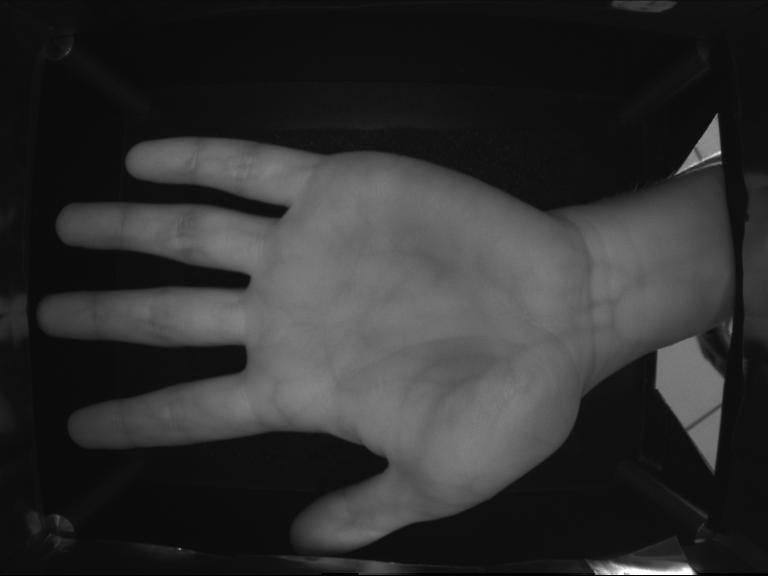
\includegraphics[width=\textwidth]{./images/preprocessing/selected_image.jpg}
            \caption{Input Image selected for preprocessing.}
            \label{fig:selected_image}
        \end{subfigure}
        \hfill
        \begin{subfigure}[t]{0.48\columnwidth}
            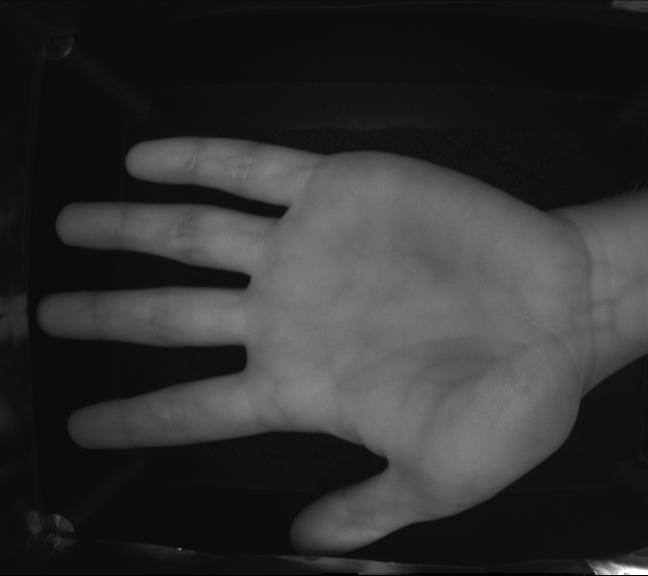
\includegraphics[width=\textwidth]{./images/preprocessing/cropped_image.png}
            \caption{Cropped Image after removing the rightmost part.} 
            \label{fig:cropped_image}
        \end{subfigure}
    \end{figure}

    \item \textbf{Blurring and Thresholding}
    A Gaussian blur was applied to smooth the image and reduce noise and Thresholding was then applied to convert the image to binary format:
    \begin{equation}
        I_{\text{thresholded}}(x, y) =
        \begin{cases}
        255 & \text{if } I_{\text{blur}}(x, y) \geq T, \\
        0 & \text{if } I_{\text{blur}}(x, y) < T
        \end{cases}   
    \end{equation} 
    where \( T = 50 \).

    Figure \ref{fig:thresholded_image} shows the thresholded image after applying Gaussian blur.

    \item \textbf{Contour Detection}
    Contours were extracted from the binary image. The largest contour, corresponding to the hand region, was selected. 

    \begin{figure}[!ht]
        \centering
        \begin{subfigure}[t]{0.48\columnwidth}
            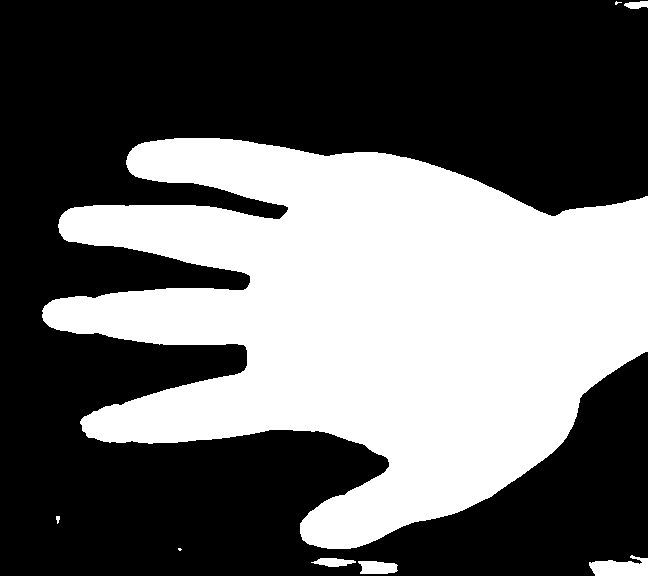
\includegraphics[width=\textwidth]{./images/preprocessing/thresholded_image.png}
            \caption{Thresholded Image after Gaussian Blur.} 
            \label{fig:thresholded_image}
        \end{subfigure}
        \hfill
        \begin{subfigure}[t]{0.48\columnwidth}
            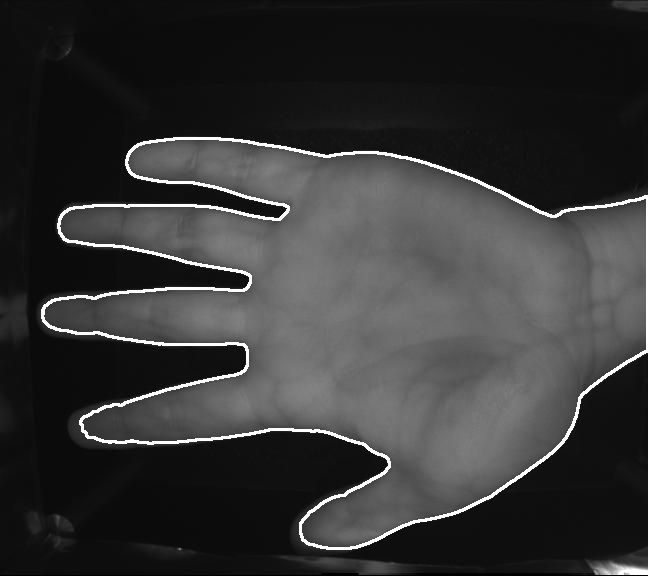
\includegraphics[width=\textwidth]{./images/preprocessing/contour_image.png}
            \caption{Contour Image after extracting contours.}
            \label{fig:contour_image}
        \end{subfigure}
    \end{figure}

    Figure \ref{fig:contour_image} shows the contour image after extracting contours.

    \item \textbf{Convexity Defects Analysis}
    The convex hull of the largest contour was calculated using the convexHull function from OpenCV described in Equation \ref{eq:convex_hull} where \( C_{\text{largest}} \) represents the largest contour.
    
    \begin{equation}
        H = \text{convexHull}(C_{\text{largest}})
        \label{eq:convex_hull}
    \end{equation}

    Convexity defects, representing regions where the contour deviates inward from the hull, were identified using OpenCV's convexityDefects function described in Equation \ref{eq:convexity_defects}.

    \begin{equation}
        D = \text{convexityDefects}(C_{\text{largest}}, H)
        \label{eq:convexity_defects}
    \end{equation}

    \item \textbf{Region of Interest (ROI) Extraction} 
    Once the convexity defects are calculated, the region of interest (ROI) is determined by identifying key farthest points from the contour, sorting them based on depth and position, and using these points to define the primary axis of interest. The midpoint and direction vector of this axis are computed, enabling the derivation of a perpendicular point. These geometric constructs are then used to generate, align, and position a square ROI.

    \begin{figure}[!ht]
        \centering
        \begin{subfigure}[t]{0.48\columnwidth}
            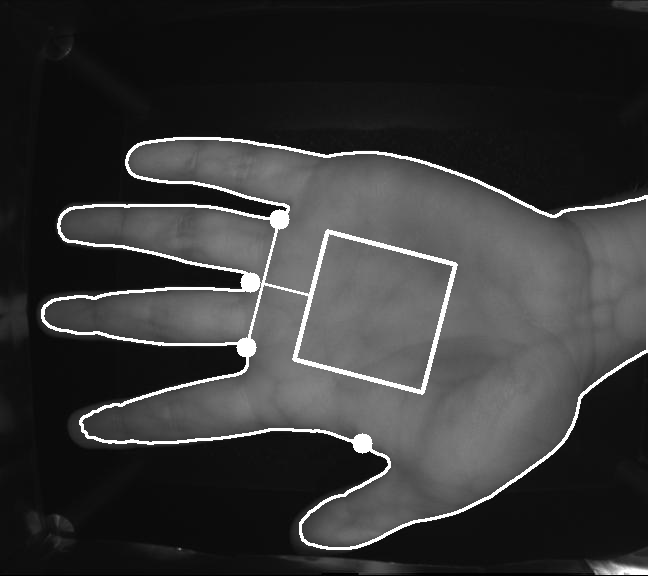
\includegraphics[width=\textwidth]{./images/preprocessing/far_points_line_perpendicular_square_image.png}
            \caption{Far Points, Line, and Perpendicular Line connected to the ROI Square.}
            \label{fig:far_points_line_perpendicular_square_image}
        \end{subfigure}
        \hfill
        \begin{subfigure}[t]{0.48\columnwidth}
            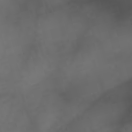
\includegraphics[width=\textwidth]{./images/preprocessing/rectified_image.png}
            \caption{ROI Area extracted from the image.}
            \label{fig:rectified_image}
        \end{subfigure}
    \end{figure}

    \item \textbf{Feature Enhancement}
    Once the region of interest (ROI) is extracted, the image undergoes histogram equalization to enhance contrast and normalize brightness variations, ensuring uniform feature representation. Following this, a Gabor filter is applied to extract texture features from the ROI.

    \begin{table}[h!]
        \centering
        \caption{Gabor Filter Parameters}
        \label{tab:gabor_params}
        \setlength{\tabcolsep}{4pt}
        \renewcommand{\arraystretch}{1.2}
        \begin{tabular}{|c|c|}
        \hline
        \textbf{Parameter} & \textbf{Value} \\ \hline
        Kernel Size ($k$)  & 5              \\ \hline
        Sigma ($\sigma$)   & 2.5            \\ \hline
        Theta ($\theta$)   & $\pi / 3$      \\ \hline
        Lambda ($\lambda$) & 8.0            \\ \hline
        Gamma ($\gamma$)   & 0.4            \\ \hline
        Psi ($\psi$)       & 0.0            \\ \hline
        \end{tabular}
    \end{table}
    
    \begin{figure}[!ht]
        \centering
        \begin{subfigure}[t]{0.48\columnwidth}
            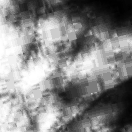
\includegraphics[width=\textwidth]{./images/preprocessing/rectified_image_equalized.png}
            \caption{Image after applying Histogram Equalization.}
            \label{fig:rectified_image_equalized}
        \end{subfigure}
        \hfill
        \begin{subfigure}[t]{0.48\columnwidth}
            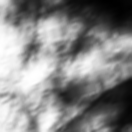
\includegraphics[width=\textwidth]{./images/preprocessing/gabor_filtered_image.png}
            \caption{Image after applying Gabor Filter.}
            \label{fig:gabor_filtered_image}
        \end{subfigure}
    \end{figure}

    \item \textbf{CLAHE}
    The contrast of the region of interest (ROI) is further enhanced using Contrast Limited Adaptive Histogram Equalization (CLAHE) and Gaussian blur. CLAHE is applied iteratively with varying tile grid sizes (\((4, 4)\), \((8, 8)\), and \((10, 10)\)) and a clip limit of 2.0, which adaptively enhances the local contrast while mitigating noise amplification. A Gaussian blur with a kernel size of \((5, 5)\) is then applied to smooth the image and reduce noise.

    \item \textbf{Binary Thresholding}
    The processed image was binarized to isolate vein patterns:
    \[
    I_{\text{binary}}(x, y) =
    \begin{cases}
    255 & \text{if } I_{\text{CLAHE}}(x, y) \geq T_{\text{final}}, \\
    0 & \text{otherwise}
    \end{cases}
    \]

    \item \textbf{Resize and Save} 
    Each image after the binary thresholding step was resized to \( 128 \times 128 \) pixels to standardize the input size for the neural network model.

    \begin{figure}[!ht]
        \centering
        \begin{subfigure}[t]{0.48\columnwidth}
            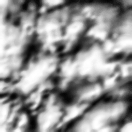
\includegraphics[width=\textwidth]{./images/preprocessing/enhanced_image.png}
            \caption{Enhanced image after Using CLAHE and Gaussian Blur.}
            \label{fig:enhanced_image}
        \end{subfigure}
        \hfill
        \begin{subfigure}[t]{0.48\columnwidth}
            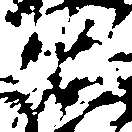
\includegraphics[width=\textwidth]{./images/preprocessing/binarize_image.png}
            \caption{Binary Thresholding of the image.}
            \label{fig:binarize_image}
        \end{subfigure}
    \end{figure}

    Figure \ref{fig:binarize_image} shows the final output of the preprocessing pipeline.
\end{enumerate}

\subsection{Model Architecture}
Convolutional Neural Networks (CNNs) are a class of deep learning models specifically designed to process and analyze grid-like data such as images. They use layers of convolutional filters to automatically detect and learn hierarchical patterns in the data, making them particularly effective for image recognition and classification tasks \cite{726791}.

The structure of the neural network models developed for the palm vein identification system is detailed here. These models share a similar core structure, with differences in specific components to address their respective objectives: closed-set identification, open-set identification, and verification.

\textbf{Core Structure}: Both models rely on the same convolutional backbone for feature extraction. This shared structure consists of four convolutional layers that extract features from the input image. Each convolutional layer increases the number of feature maps while reducing spatial dimensions using ReLU activation Function \ref{eq:relu} followed by max pooling Function \ref{eq:maxpool}. After the convolutional layers, the flattened feature maps are passed through a linear layer to produce a 128-dimensional representation of the image features. This linear layer, acting as a dense fully connected layer, is essential for transforming the high-dimensional convolutional features into a compact representation suitable for further processing.

\begin{equation}
    f(x) = \max(0, x)
    \label{eq:relu}
\end{equation}

\begin{equation}
    y_{i,j} = \max_{(m,n) \in R_{i,j}} x_{m,n}
    \label{eq:maxpool}
\end{equation}

\textbf{Model 1} The CNN Model Architecture presented in Figure \ref{fig:model-1} is used for the Open and Closed Set Identification. Designed with the goal of identifying a predefined number of classes, such as 100 patients, this model uses a shared backbone to extract features from the input image. The model then uses a linear layer to reduce the dimensionality of the features, followed by a fully connected layer to output class predictions using a softmax activation function. 

\begin{figure}[ht!]
    \centering
    \begin{tikzpicture}[
        font=\sffamily,
        node distance=0.6cm and 1.5cm,
        scale=0.6,
        transform shape,
        >={Stealth[open]},
        every node/.style={align=center},
        conv/.style={draw, minimum width=2cm, minimum height=1cm, rounded corners, fill=blue!10},
        relu/.style={draw, minimum width=2cm, minimum height=1cm, rounded corners, fill=green!10},
        pool/.style={draw, minimum width=2cm, minimum height=1cm, rounded corners, fill=yellow!10},
        linear/.style={draw, minimum width=2cm, minimum height=1cm, rounded corners, fill=orange!10},
        fc/.style={draw, minimum width=2cm, minimum height=1cm, rounded corners, fill=red!10},
        drop/.style={draw, dashed, minimum width=2cm, minimum height=1cm, rounded corners, fill=gray!10},
        softmax/.style={draw, minimum width=2cm, minimum height=1cm, rounded corners, fill=purple!10},
        input/.style={font=\large},
        output/.style={draw, minimum width=2cm, minimum height=1cm, rounded corners, fill=cyan!10, font=\large}
    ]
    \node[input] (input) {Input \\ $128 \times 128$};
    \node[conv, below=of input] (conv1) {Conv1 \\ $16@128 \times 128$};
    \node[relu, below=of conv1] (relu1) {ReLU};
    \node[pool, below=of relu1] (pool1) {MaxPool \\ $2\times 2$};
    \node[conv, below=of pool1] (conv2) {Conv2 \\ $32@64 \times 64$};
    \node[relu, below=of conv2] (relu2) {ReLU};
    \node[pool, below=of relu2] (pool2) {MaxPool \\ $2\times 2$};
    
    \node[conv, right=3cm of input] (conv3) {Conv3 \\ $64@32 \times 32$};
    \node[relu, below=of conv3] (relu3) {ReLU};
    \node[pool, below=of relu3] (pool3) {MaxPool \\ $2\times 2$};
    \node[conv, below=of pool3] (conv4) {Conv4 \\ $128@16 \times 16$};
    \node[relu, below=of conv4] (relu4) {ReLU};
    \node[linear, below=of relu4] (linear1) {Linear \\ Flatten to $32*32*32$};

    \node[fc, right=3cm of conv3] (fc1) {FC1 \\ 128};
    \node[drop, below=of fc1] (drop1) {Dropout \\ 0.5};
    \node[linear, below=of drop1] (linear2) {Linear \\ $128 \to \text{Num Classes}$};
    \node[fc, below=of linear2] (fc2) {FC2 \\ Num Classes};
    \node[softmax, below=of fc2] (softmax) {Softmax};
    \node[output, below=of softmax] (output) {Output \\ Class Predictions};

    \draw[->] (input.south) -- (conv1.north);
    \draw[->] (conv1.south) -- (relu1.north);
    \draw[->] (relu1.south) -- (pool1.north);
    \draw[->] (pool1.south) -- (conv2.north);
    \draw[->] (conv2.south) -- (relu2.north);
    \draw[->] (relu2.south) -- (pool2.north);
    \draw[->] (pool2.east) -- ++(1.0,0) |- (conv3.west);
    \draw[->] (conv3.south) -- (relu3.north);
    \draw[->] (relu3.south) -- (pool3.north);
    \draw[->] (pool3.south) -- (conv4.north);
    \draw[->] (conv4.south) -- (relu4.north);
    \draw[->] (relu4.south) -- (linear1.north);

    \draw[->] (linear1.east) -- ++(1.0,0) |- (fc1.west);
    \draw[->] (fc1.south) -- (drop1.north);
    \draw[->] (drop1.south) -- (linear2.north);
    \draw[->] (linear2.south) -- (fc2.north);
    \draw[->] (fc2.south) -- (softmax.north);
    \draw[->] (softmax.south) -- (output.north);

    \end{tikzpicture}
    \caption{Forward Pass of the CNN Model used for the Open and Closed Set Identification.}
    \label{fig:model-1}
\end{figure}

\textbf{Model 2} The CNN Model Architecture presented in Figure \ref{fig:model-2} is used for Verification. Designed with the goal of verifiying the authenticity of a given image-label pair, this model uses a shared backbone to extract features from the input image. The model then uses a linear layer to extract a compact feature representation, followed by label embeddings to capture label-specific information. It concatenates the 128-dimensional image features with the label embeddings to form a combined 256-dimensional vector. This fused representation is passed through a fully connected layer and sigmoid activation to output a verification score between 0 and 1, indicating the likelihood of a valid image-label pair.

\begin{figure}[h!]
    \centering
    \begin{tikzpicture}[
        font=\sffamily,
        node distance=0.6cm and 1.5cm,
        scale=0.6,
        transform shape,
        >={Stealth[open]},
        every node/.style={align=center},
        conv/.style={draw, minimum width=1.5cm, minimum height=0.8cm, rounded corners, fill=blue!10},
        relu/.style={draw, minimum width=1.5cm, minimum height=0.8cm, rounded corners, fill=green!10},
        pool/.style={draw, minimum width=1.5cm, minimum height=0.8cm, rounded corners, fill=yellow!10},
        embed/.style={draw, minimum width=1.5cm, minimum height=0.8cm, rounded corners, fill=orange!10},
        linear/.style={draw, minimum width=1.5cm, minimum height=0.8cm, rounded corners, fill=red!10},
        concat/.style={draw, minimum width=1.5cm, minimum height=0.8cm, rounded corners, fill=purple!10},
        sigmoid/.style={draw, minimum width=1.5cm, minimum height=0.8cm, rounded corners, fill=gray!10},
        input/.style={font=\large},
        output/.style={draw, minimum width=1.5cm, minimum height=0.8cm, rounded corners, fill=cyan!10}
    ]
    \node[input] (image_input) {Input Image \\ $128 \times 128$};
    \node[conv, below=of image_input] (conv1) {Conv1 \\ $16@128 \times 128$};
    \node[relu, below=of conv1] (relu1) {ReLU};
    \node[pool, below=of relu1] (pool1) {MaxPool \\ $2\times 2$};
    \node[conv, below=of pool1] (conv2) {Conv2 \\ $32@64 \times 64$};
    \node[relu, below=of conv2] (relu2) {ReLU};
    \node[pool, below=of relu2] (pool2) {MaxPool \\ $2\times 2$};
    \node[conv, right=3cm of image_input] (conv3) {Conv3 \\ $64@32 \times 32$};
    \node[relu, below=of conv3] (relu3) {ReLU};
    \node[pool, below=of relu3] (pool3) {MaxPool \\ $2\times 2$};
    \node[conv, below=of pool3] (conv4) {Conv4 \\ $128@16 \times 16$};
    \node[relu, below=of conv4] (relu4) {ReLU};
    \node[linear, below=of relu4] (linear1) {Linear1 \\ Transform $128 \to 128$};
    \node[linear, below=of linear1] (fc_image) {FC Image \\ 128 Features};
    \node[input, right=3cm of conv3] (label_input) {Label \\ One-hot};
    \node[embed, below=of label_input] (label_embed) {Label Embedding \\ 128 Features};
    \node[concat, below=of label_embed, yshift=-0.5cm] (concat) {Concatenation \\ $128 + 128$};
    \node[linear, below=of concat, yshift=-0.5cm] (linear2) {Linear2 \\ $256 \to 128$};
    \node[linear, below=of linear2, yshift=-0.5cm] (fc_final) {FC Final \\ $128 \to 1$};
    \node[sigmoid, below=of fc_final, yshift=-0.5cm] (output) {Output \\ Sigmoid};

    \draw[->] (image_input.south) -- (conv1.north);
    \draw[->] (conv1.south) -- (relu1.north);
    \draw[->] (relu1.south) -- (pool1.north);
    \draw[->] (pool1.south) -- (conv2.north);
    \draw[->] (conv2.south) -- (relu2.north);
    \draw[->] (relu2.south) -- (pool2.north);
    \draw[->] (pool2.east) -- ++(1.0,0) |- (conv3.west);
    \draw[->] (conv3.south) -- (relu3.north);
    \draw[->] (relu3.south) -- (pool3.north);
    \draw[->] (pool3.south) -- (conv4.north);
    \draw[->] (conv4.south) -- (relu4.north);
    \draw[->] (relu4.south) -- (linear1.north);
    \draw[->] (linear1.south) -- (fc_image.north);
    \draw[->] (label_input.south) -- (label_embed.north);
    \draw[->] (fc_image.east) -- ++(1.0,0) |- (concat.west);
    \draw[->] (label_embed.south) -- ++(0,-0.8) -| (concat.north);
    \draw[->] (concat.south) -- (linear2.north);
    \draw[->] (linear2.south) -- (fc_final.north);
    \draw[->] (fc_final.south) -- (output.north);

    \end{tikzpicture}
    \caption{Forward Pass of the CNN Model used for Verification.}
    \label{fig:model-2}
\end{figure}
